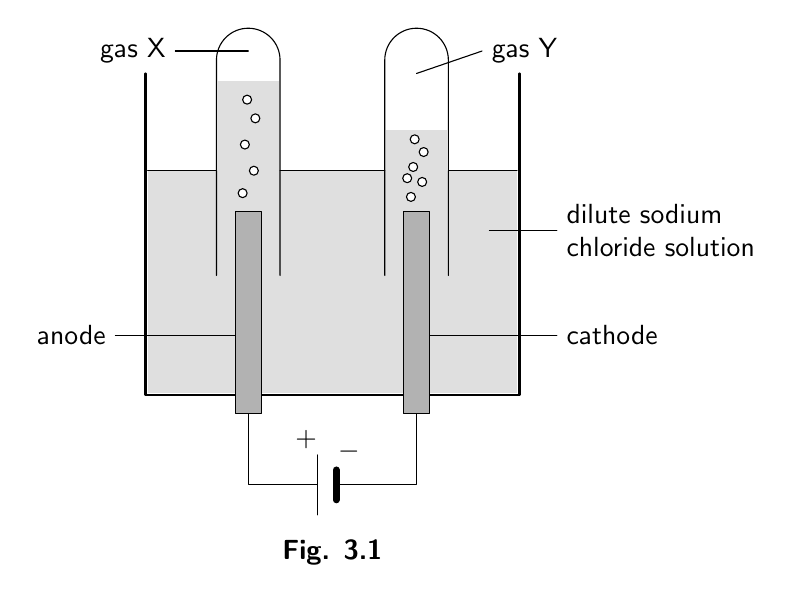
\begin{tikzpicture}[scale=0.95, font=\sffamily, line join=round, line cap=round]
  % electrolyte
  \fill[gray!25] (0.03,0.03) rectangle (4.97,3.0);
  % liquid trapped inside each tube (gas collects above)
  \fill[gray!25] (0.97,2.95) rectangle (1.78,4.2);   % anode tube: less gas
  \fill[gray!25] (3.22,2.95) rectangle (4.03,3.55);  % cathode tube: twice the gas
  \draw (0.03,3.0)--(0.95,3.0) (1.8,3.0)--(3.2,3.0) (4.05,3.0)--(4.97,3.0);
  % beaker
  \draw[thick] (0,4.3)--(0,0)--(5,0)--(5,4.3);
  % inverted test tubes
  \draw (0.95,1.6)--(0.95,4.48) arc (180:0:0.425)--(1.8,1.6);
  \draw (3.2,1.6)--(3.2,4.48) arc (180:0:0.425)--(4.05,1.6);
  % carbon electrodes
  \draw[fill=gray!60] (1.2,-0.25) rectangle (1.55,2.45);
  \draw[fill=gray!60] (3.45,-0.25) rectangle (3.8,2.45);
  % bubbles
  \foreach \p in {(1.3,2.7),(1.45,3.0),(1.33,3.35),(1.47,3.7),(1.36,3.95)} \draw[fill=white] \p circle (0.06);
  \foreach \p in {(3.55,2.65),(3.7,2.85),(3.58,3.05),(3.72,3.25),(3.6,3.42),(3.5,2.9)} \draw[fill=white] \p circle (0.06);
  % circuit
  \draw (1.375,-0.25)--(1.375,-1.2)--(2.3,-1.2);
  \draw (2.55,-1.2)--(3.625,-1.2)--(3.625,-0.25);
  \draw (2.3,-1.6)--(2.3,-0.8);
  \draw[line width=2.5pt] (2.55,-1.4)--(2.55,-1.0);
  \node at (2.15,-0.6) {$+$};
  \node at (2.72,-0.75) {$-$};
  % labels
  \draw (1.375,4.6)--(0.4,4.6) node[left] {gas X};
  \draw (3.625,4.3)--(4.5,4.6) node[right] {gas Y};
  \draw (1.2,0.8)--(-0.4,0.8) node[left] {anode};
  \draw (3.8,0.8)--(5.5,0.8) node[right] {cathode};
  \draw (4.6,2.2)--(5.5,2.2) node[right, align=left] {dilute sodium\\chloride solution};
  \node[font=\sffamily\bfseries] at (2.5,-2.1) {Fig. 3.1};
\end{tikzpicture}
